%%%%%%%%%%%%%%%%%%%%%%%%%%%%%%%%%%%%%%%%%%%%%%%%%%%%%%%%%%%%%%%%%%%%%%%%
\chapter{REQUISITOS}
\label{ch:requisitos}
En este capítulo se presentan los requisitos a cumplir por la aplicación. Comenzaremos explicando el escenario al que pertenece la aplicación y terminaremos presentando las historias de uso de la misma.
\section{Escenario}

En el contexto de este trabajo de fin de carrera, un escenario es una descripción concreta del comportamiento de la aplicación en una determinada situación. El escenario general que se pretende cubrir con la aplicación es la posibilidad de navegar y realizar apuestas sobre eventos deportivos del portal Betfair.com. Se pretende cubrir las funcionalidades básicas que ofrece Betfair en su portal web para poder realizar apuestas y la posibilidad de realizar \emph{tranding} en las apuestas realizadas.

\section{Historias de usuario}
 Una de las formas de describir los requisitos es mediante la técnica de historias de uso. Son una representación de un requisito de software en una o dos frases usando un lenguaje común al usuario.
 
\subsection{Instalación} Para poder instalar la aplicación sólo se necesitará una cuenta del programa iTunes Store de Apple. La aplicación estará disponible para su descarga dentro de la tienda de aplicaciones  \emph{App Store} del dispositivo.  Alternativamente se podrá descargar también desde el programa iTunes para Windows y Mac. 
\subsection{Actualizar la aplicación}
La aplicación  \emph{App Store}  del dispositivo será la encargada de comunicar al usuario la aparición de una nueva versión del aplicativo. Para actualizarla simplemente habrá que seguir las indicaciones de dicho programa. %\fxnote{Lo mismo  de antes}

\subsection{Desinstalar}
Para desinstalar la aplicación simplemente se mantiene pulsado el icono de la misma unos segundos hasta que el icono empiece a vibrar. Inmediatamente pulsamos sobre el botón \textsf{X} que aparecerá es la esquina superior izquierda del icono de la aplicación. 
\subsection{Ejecución}
Para lanzar la aplicación sólo hay que pulsar el icono que aparece en la pantalla principal del dispositivo.
\subsection{Configurar la aplicación}
Se podrán configurar los diferentes aspectos de la aplicación tales como el idioma o las credenciales de acceso del  usuario a través del menú de ajustes del dispositivo. 
\begin{figure}[H]
    \centering
       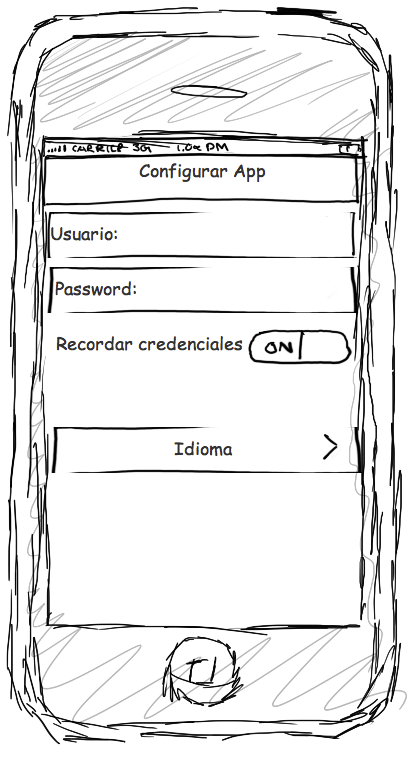
\includegraphics[width=0.3\textwidth]{./images/req_conf_app.png}
   \label{fig:Requisito configurar la aplicación}
\end{figure}
\subsection{Gestión de los eventos}
Se podrá navegar y obtener información de todos los eventos deportivos disponibles del portal Betfair. La aplicación ha de representar la información a través una jerarquía descendiente desde eventos hacia mercados de Betfair siguiendo las hojas de estilo de la interfaz de usuario de Apple.
\begin{figure}[H]
    \centering
       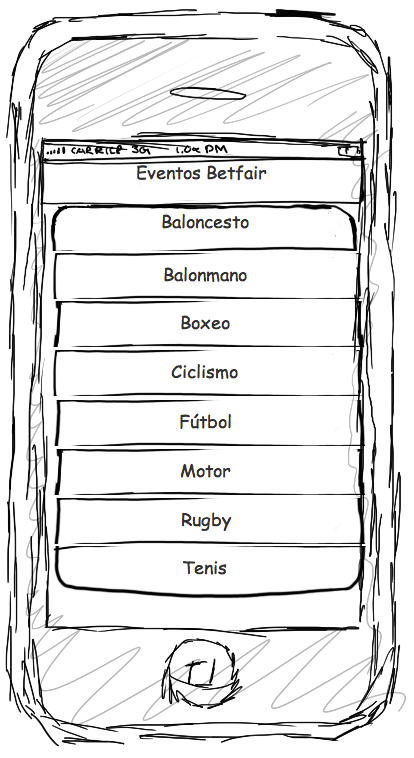
\includegraphics[width=0.3\textwidth]{./images/req_eventos.png}
   \label{fig:Requisito eventos}
\end{figure}
\subsection{Realizar una apuesta}
La aplicación permitirá la realización de una apuesta sobre un mercado específico incluyendo la cantidad y cuota deseada. El sistema notificará al usuario el resultado de la operación.
\begin{figure}[H]
    \centering
       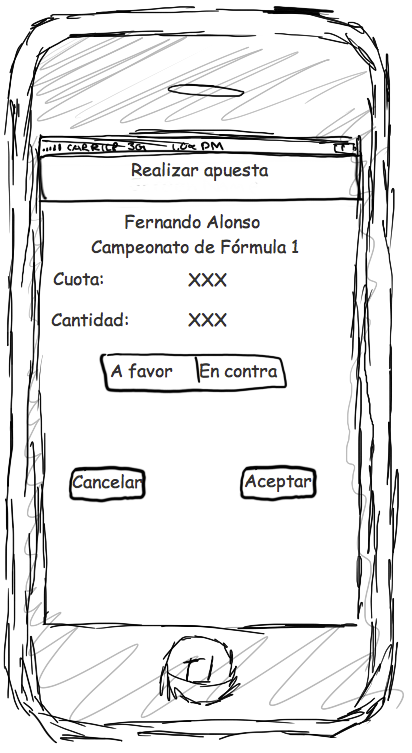
\includegraphics[width=0.3\textwidth]{./images/req_apuestas.png}
   \label{fig:Requisito realizar una apuesta}
\end{figure}
\subsection{Gestionar las apuestas}
La aplicación será capaz de recopilar todas las apuestas realizadas por el usuario sobre Betfair. Por cada apuesta, el sistema mostrará la información detallada de la apuesta, asesoramiento para \emph{trading} y estado actual del mercado.
\begin{figure}[H]
    \centering
       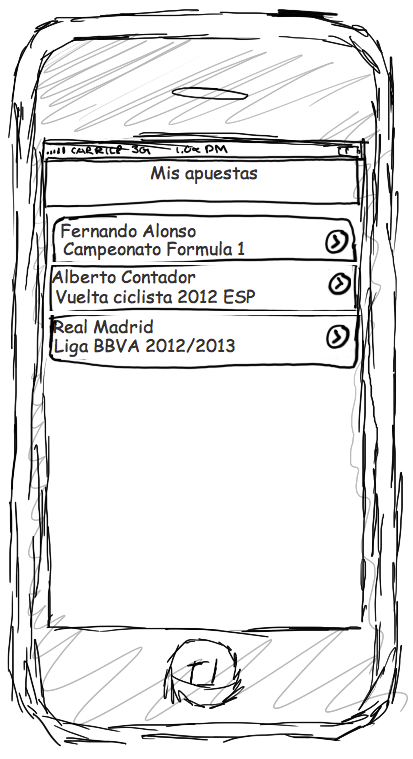
\includegraphics[width=0.3\textwidth]{./images/req_misapuestas.png}
   \label{fig:Requisito gestionar mis apuestas}
\end{figure}
\subsection{Realizar \emph{trading} sobre una apuesta ya realizada}
El sistema será capaz de asesorar para realizar \emph{trading} sobre una apuesta ya realizada anteriormente. La aplicación recomendará la apuesta más asequible a las condiciones del mercado. Se  podrá configurar la aplicación para que el \emph{trading} se realice de manera automática.
\begin{figure}[H]
    \centering
       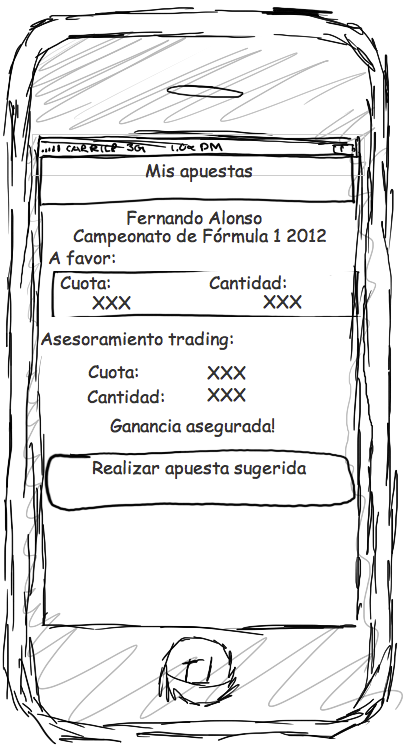
\includegraphics[width=0.3\textwidth]{./images/req_trading.png}
   \label{fig:Requisito trading}
\end{figure}

%%% Local Variables: 
%%% mode: latex
%%% TeX-master: "tfc-betfair-ios"
%%% TeX-PDF-mode: t
%%% ispell-local-dictionary: "castellano"
%%% End: 
